	\chapter{Electronics}
		This chapter provides an overview of the electronic hardware located on, and related to \index{BaralabaBob}BaralabaBob.
		\pagebreak
		
		\section{Control Boards}
        	\label{Controllers}
            \index{controllers}
			There are two main control boards on this circuit, the \index{SCC-32}SCC-32 Servo Controller, and the \index{Raspberry Pi}\index{RPi}Raspberry Pi Model B.
			
			\subsection{SCC-32 Servo Controller}
				This board came with the original purchase of the APod. It can control up to 32 servos and can be interfaced with using serial.\\
				
				\textbf{Links:}\\
				\href{http://www.lynxmotion.com/p-395-ssc-32-servo-controller.aspx}{Product Page}\\
				\href{http://www.lynxmotion.com/s/html/build136.htm}{Documentation}
				
			\subsection{Raspberry Pi Model B}
            	\index{RPi}
				This is the central brains of the robot. Originally BaralabaBob was powered by a BotBoarduino board, however I quickly realized that it would be a good idea to swap that out with an RPi for ease of programming, and the immense power having an embedded computer on it brings.
                
                I currently have two RPi V2s in stock, however I haven't had a chance to fully create their OS image to use on the robot. Because the current RPi is doing the job sufficiently, I haven't needed to upgrade to its quad-core alternatives.
				
                \index{pinout}
				\centerline{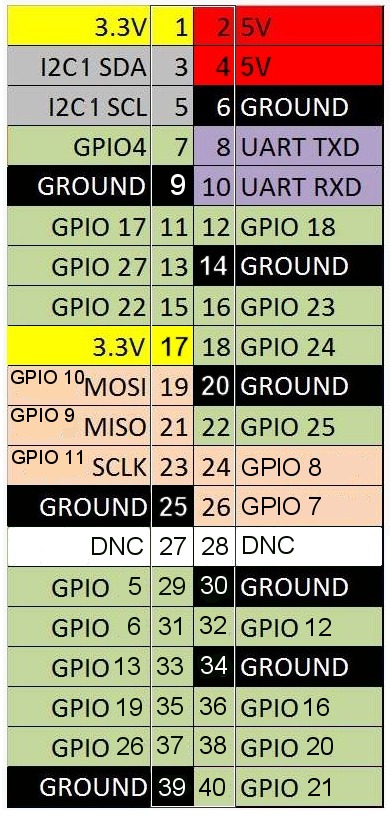
\includegraphics[width=0.5\linewidth]{rpi_pinout}}
                \vspace{10pt}
				
				\subsubsection{Storage}
                	\index{storage}\index{sd}\index{SD card}
					On BaralabaBob we are running a SanDisk Ultra (Class 10) 32GB. Previous to this I used all kinds of cheapo SD cards and had nothing but frustration with corruption and the like.\\
					
					One mistake in purchasing this was, I should have bought the micro version (which costs the same). With the advent of the release of RPi v2, I’m unable to use this SD card with it, but if I had purchased the micro version, I wouldn’t have had any issues.\\
					
				\subsubsection{Previous Controllers}
        
                	\label{BotBoarduino}
                    \index{BotBoarduino}
					Previously \index{BaralabaBob}BaralabaBob had the BotBoarduino installed, however I replaced this with the \index{RPi}\index{Raspberry Pi}RPi Model B. This RPi was fried from some unknown reason, most likely due to power spike or short circuit. We then ordered two more RPis from Pi Australia (from what I gather, associated to Little Bird Electronics) 
					\pagebreak
	
	
		\section{Power Supply}
        	\index{power supply}
            \index{batteries}
            \index{lab power supply}
			The suggested power supply was a rechargeable 6v NiMH battery. Because of the Goombungee show, and it's long term power requirements we decided to purchase a Lab Power Supply.
			
			\subsection{Lab Power Supply}
				We purchased a \href{http://www.manson.com.hk/products/detail/159}{HCS - 3402 Manson Power Supply} from 
				\href{http://www.altronics.com.au/p/m8213-manson-1-30v-20a-regulated-lab-power-supply/}{Altronics} to supply the power requirements of the Goombungee Show.
				
				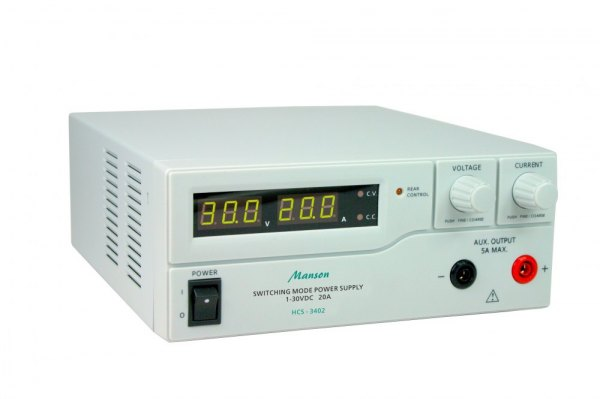
\includegraphics[width=\linewidth]{power_supply}
			
			\subsection{Battery}
            	There are two batteries on-board the robot. The reason behind this is, when 25 servo motors start up on the main power supply, it causes many ripples and drops the voltage way below the brownout threshold of the \index{microcontroller}microcontroller.\\
                
                \centerline{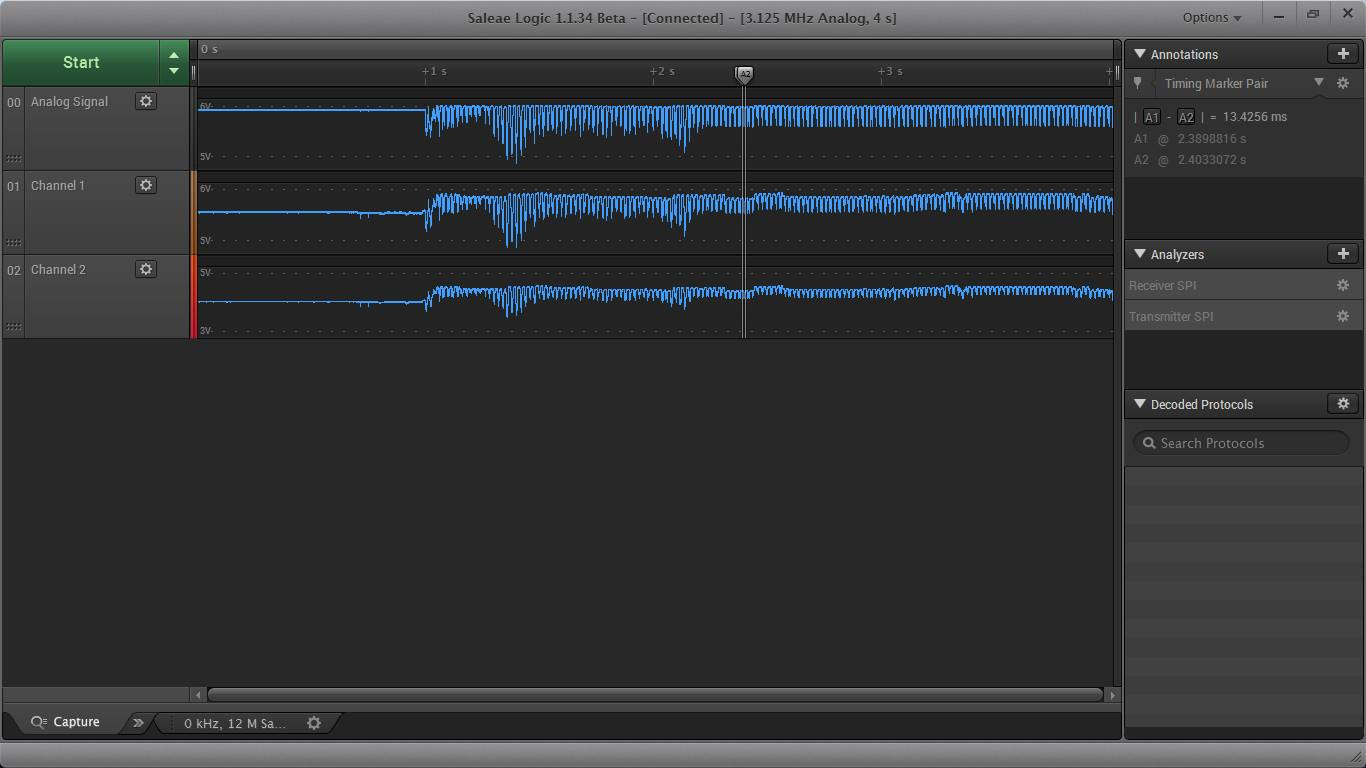
\includegraphics[width=0.75\linewidth]{power_supply_graph}}
                \vspace{10pt}
                
                \index{power circuit}
                I tried designing a power circuit (as seen on the back of the robot) to try and counter this, but it was unsuccessful, as the brownout was too severe for too long a time. The circuit consists of capacitor/diode pairs (whilst power is good the caps power up, then when power goes bad the MCU is powered by the cap, and the diode prevents backflow of current back into the motors). The board features two output USB ports. The ports obviously don't carry data, only power.\\                                                
                \centerline{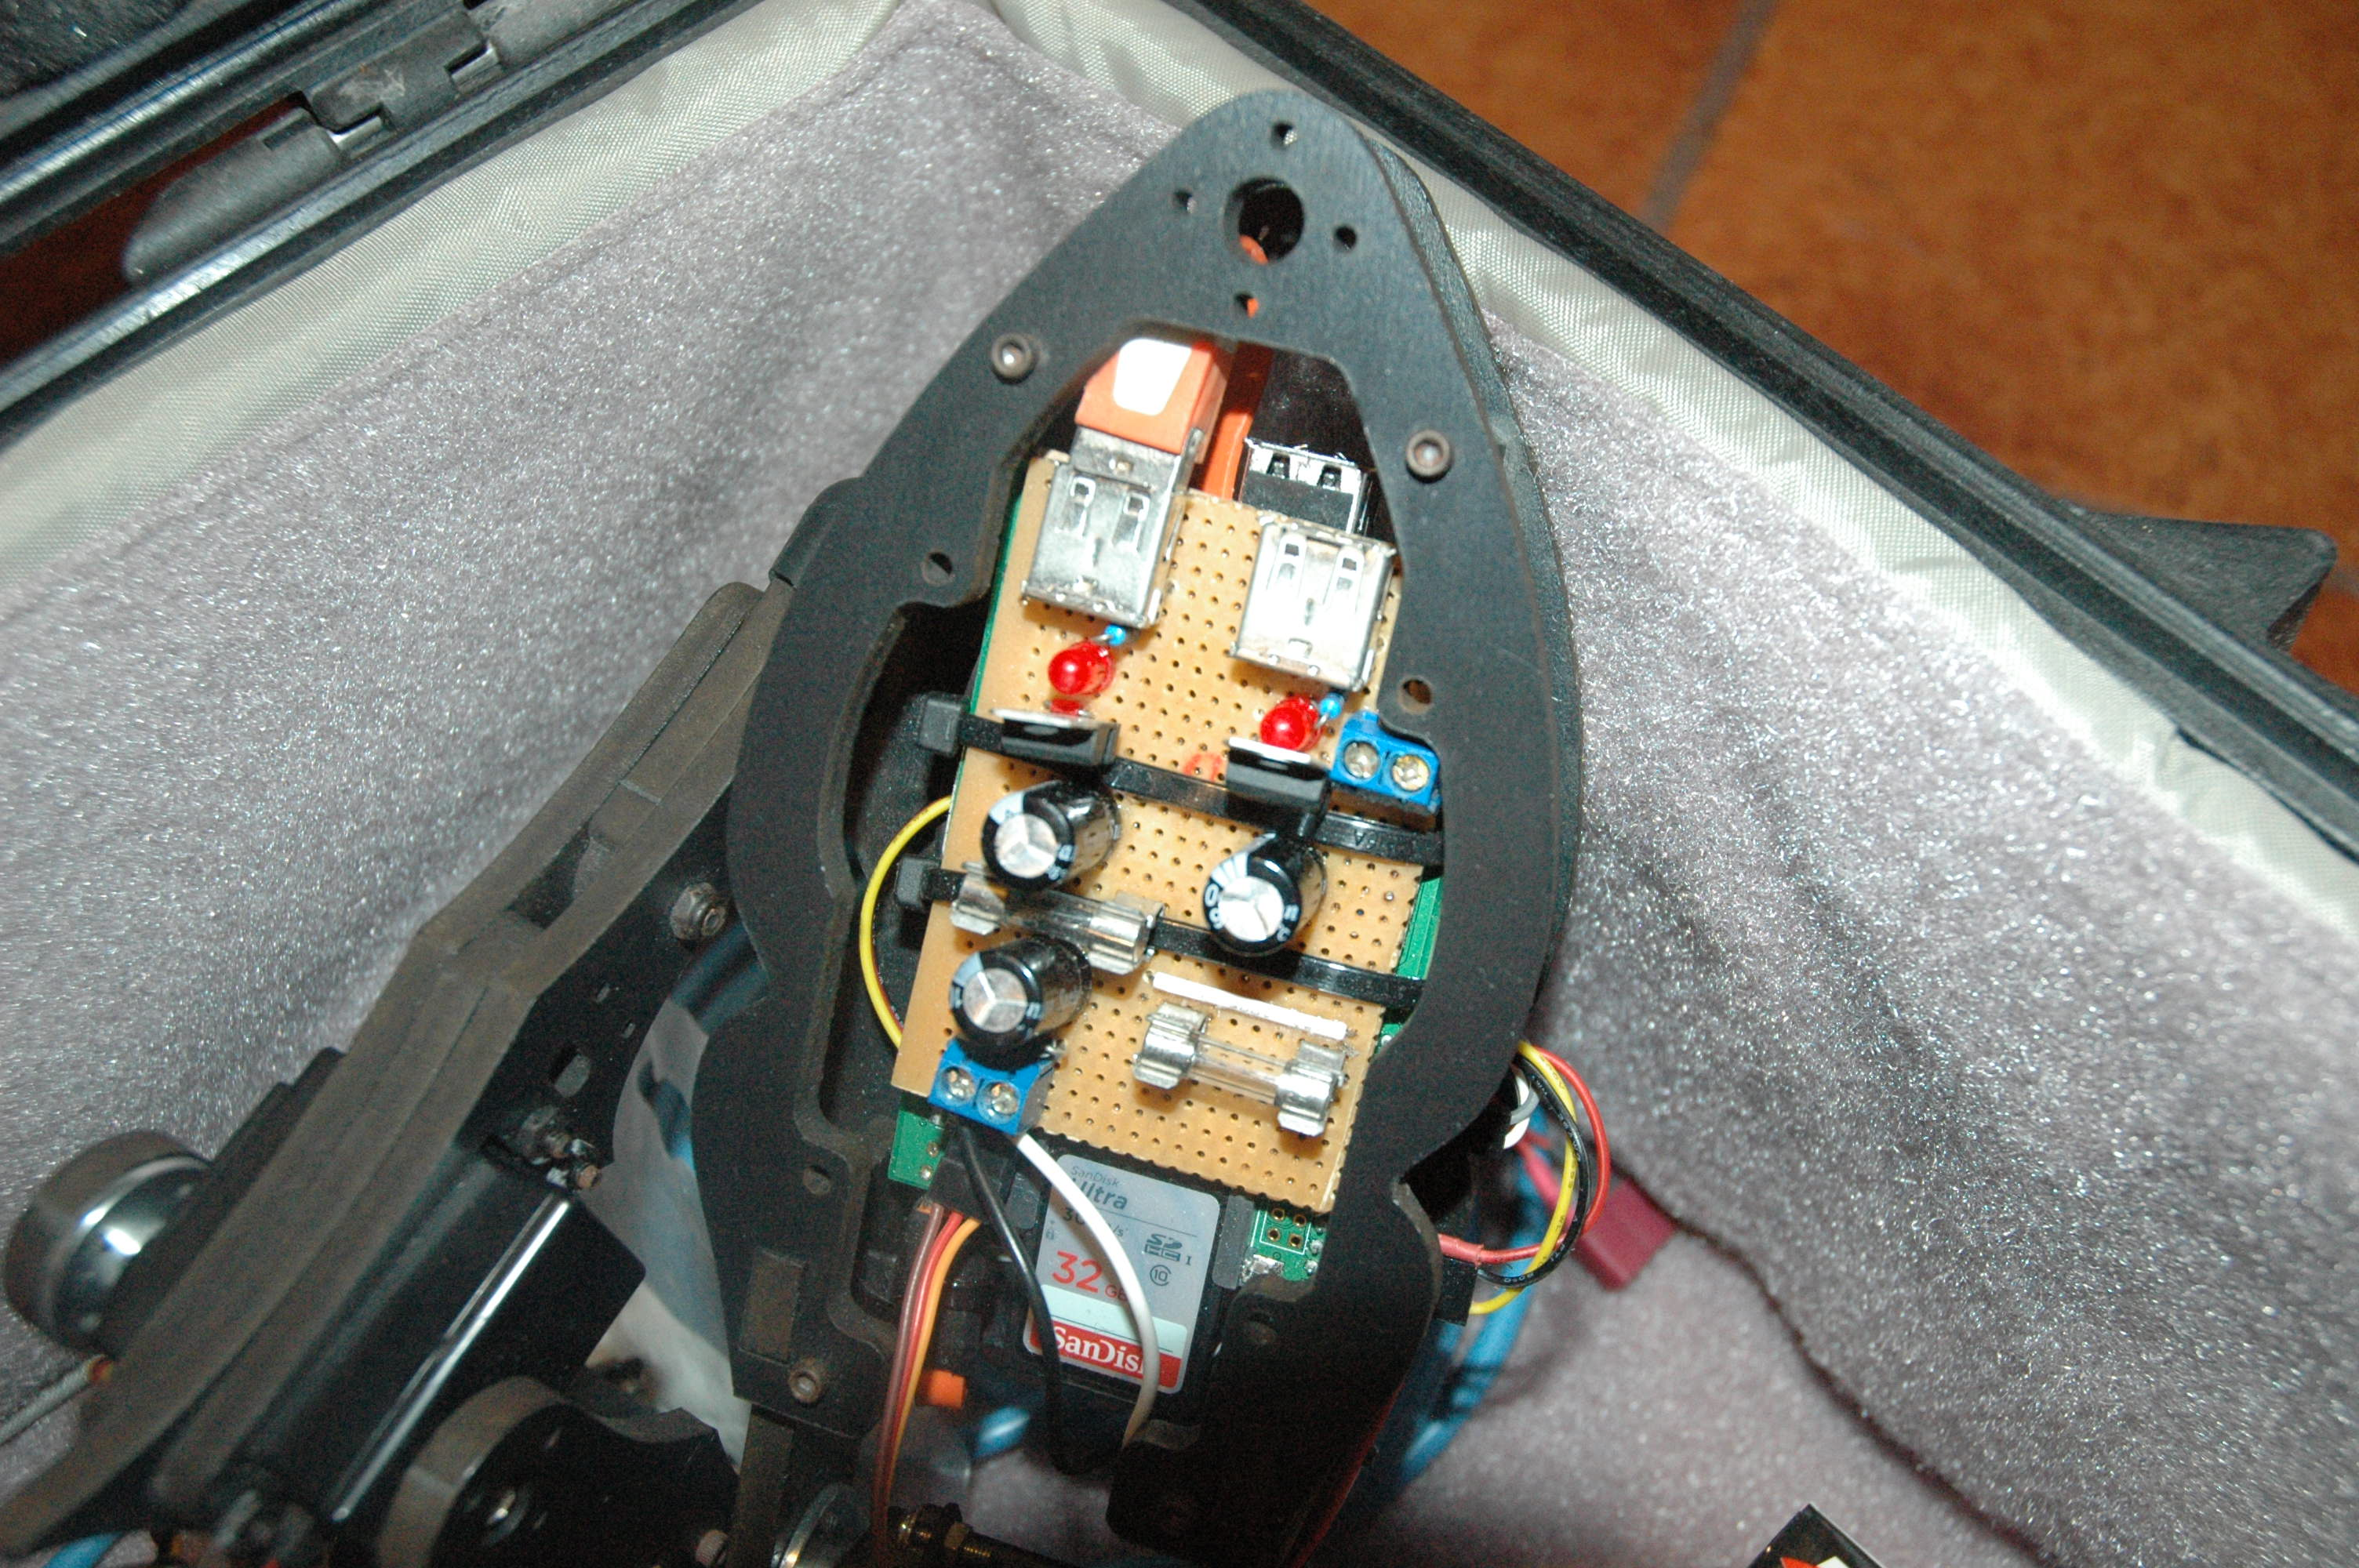
\includegraphics[width=0.75\linewidth]{power_supply_circuit}}
                \vspace{10pt}
                
                \index{brownout}
                Although the board doesn't solve the problem of brownouts, it is a very functional and flexible power distribution board. It takes in power via either header (for direct connection to small batteries) or screw terminal. It then sends this power through two identical circuits which fuse protect, regulate the voltage to 5A, give a visual indicator using a red LED, and then distribute power via USB or screw terminal.\\
                
                \index{USB}
                \index{WiFi}
                I chose USB as the power distribution connector because the RPI takes power in via a USB B-micro port. I also have the second USB power because I can use it with a y-cable to supply power to any power-hungry peripherals that I might want plugged into the RPi, such as a camera, Alfa AWUS036NHV WiFi adapter, or external hard drive.\\
                
                As for the batteries, I use one 7.2V NiMH racing car battery, and one 7.4V 500mA LiPo.\\
                
             	\centerline{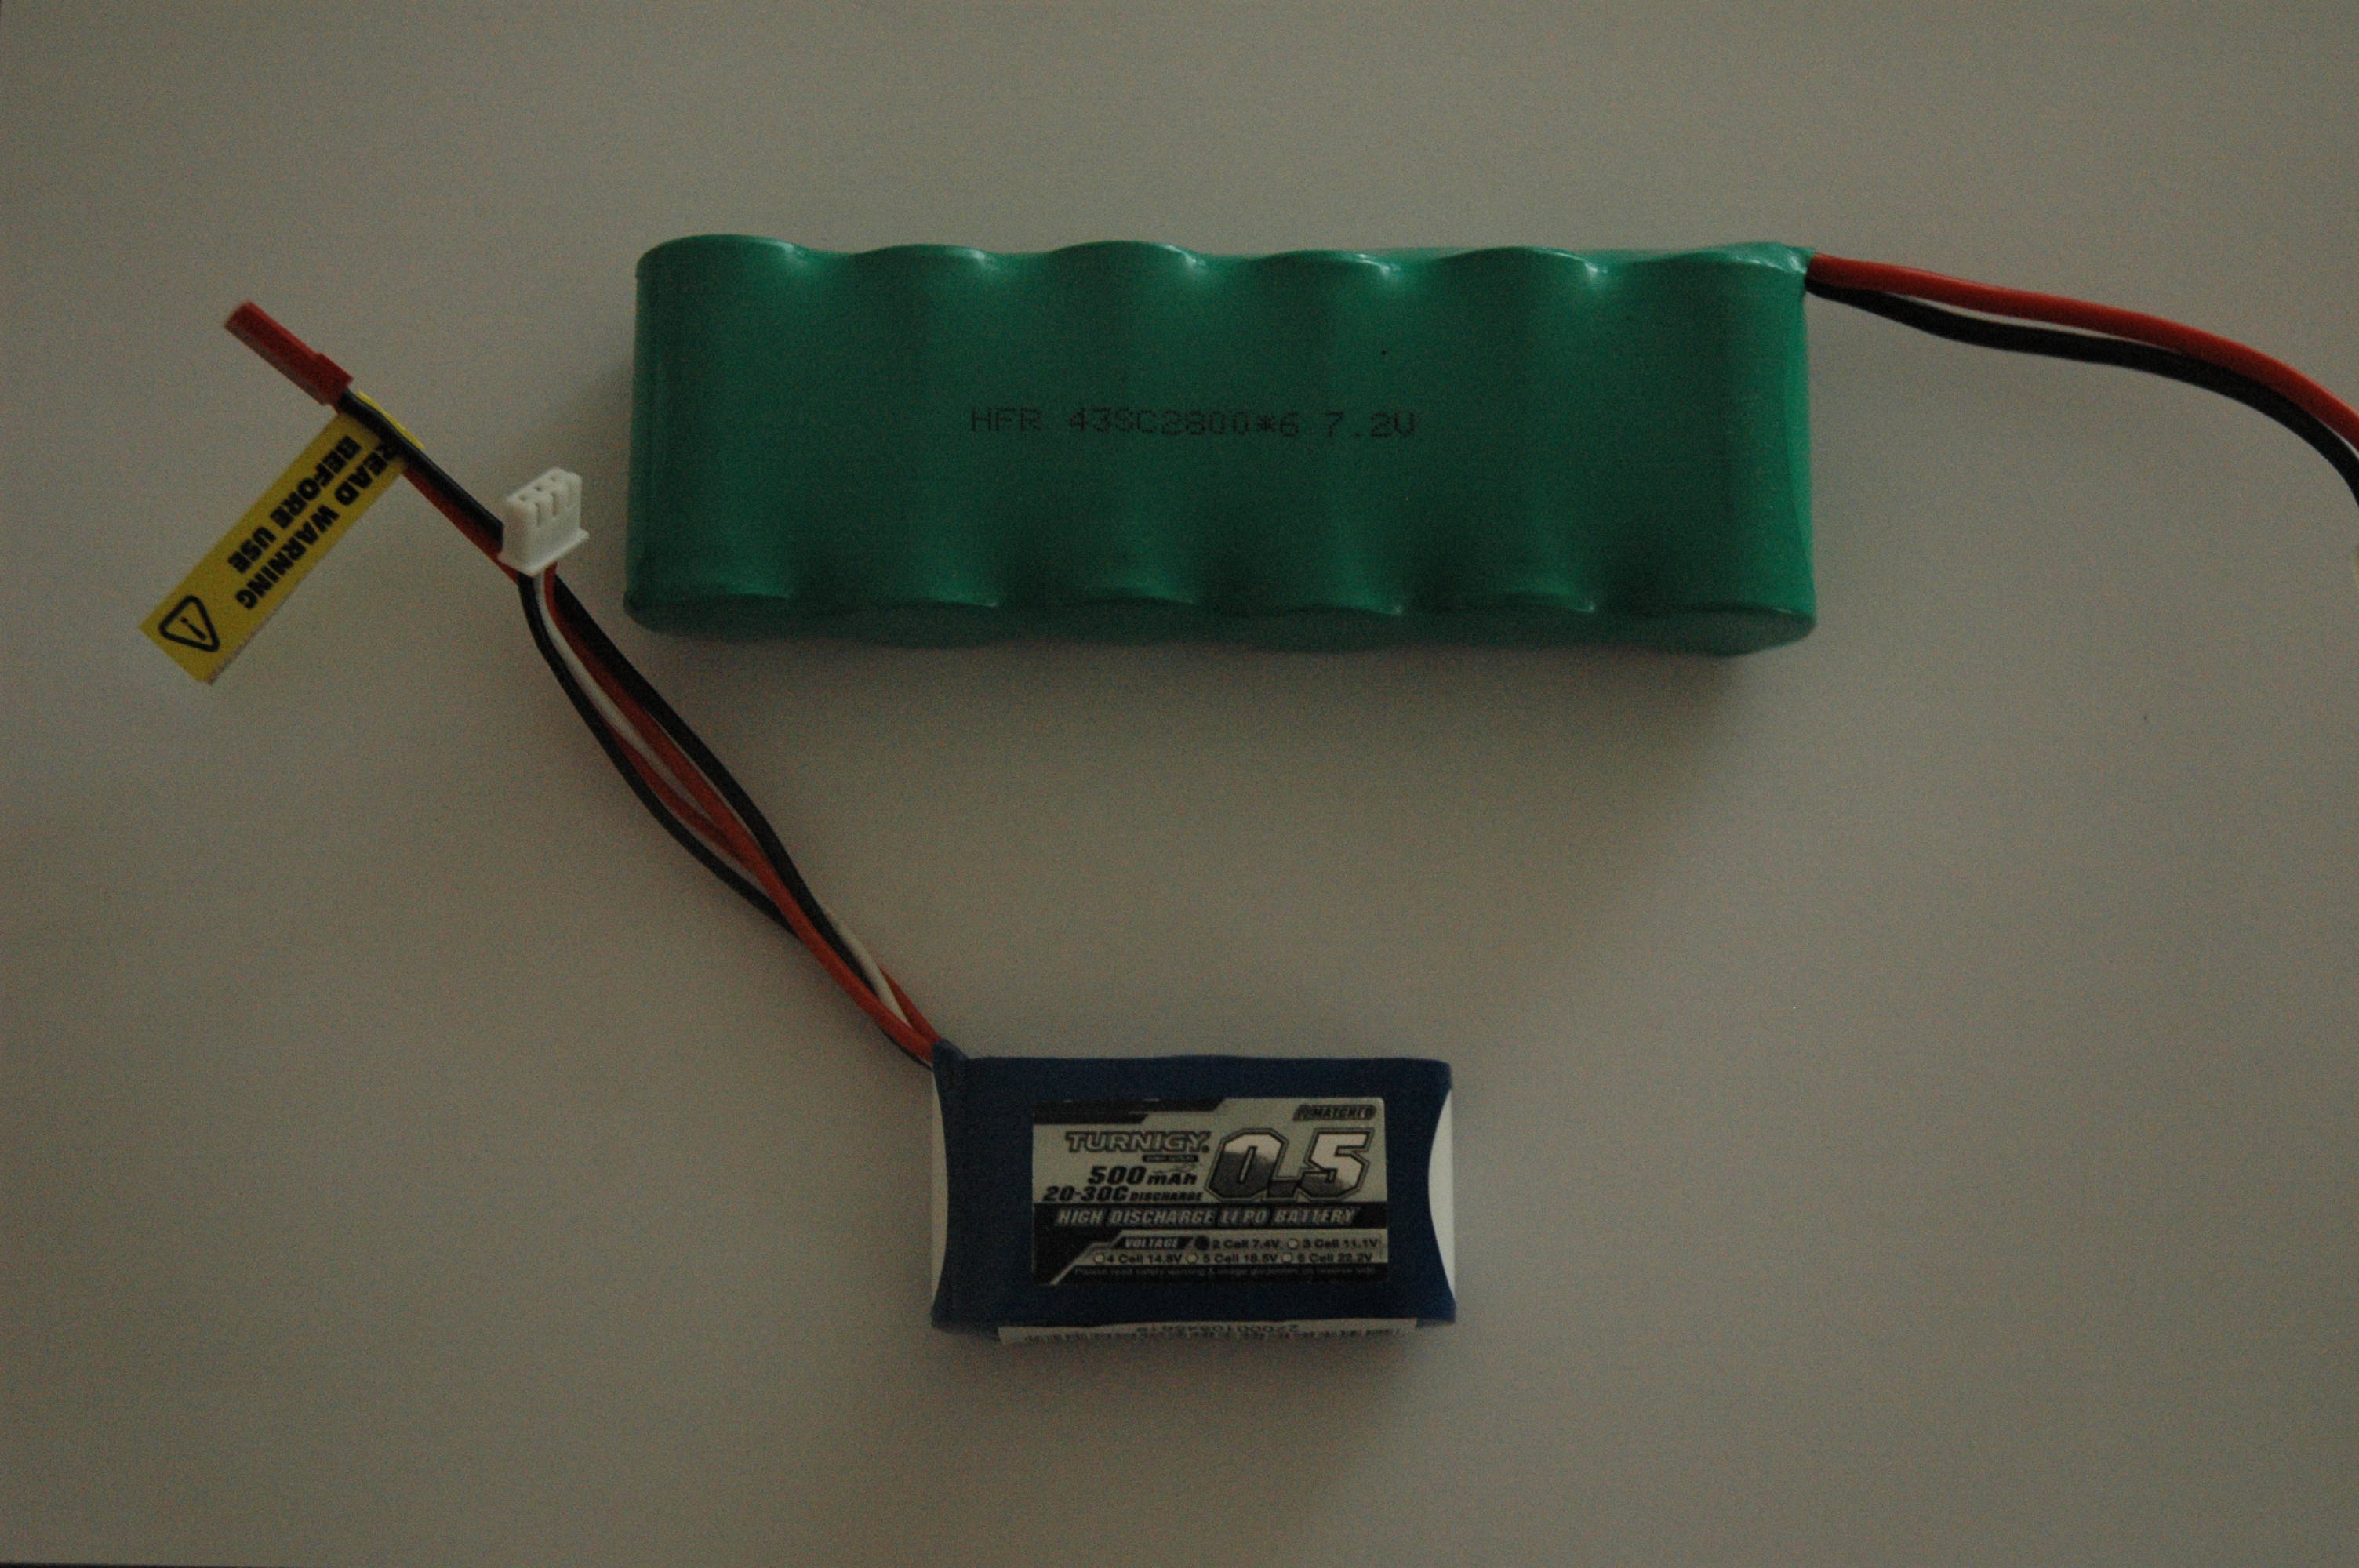
\includegraphics[width=0.75\linewidth]{batteries}}
                \vspace{10pt}
                
                \subsubsection{LiPo Disposal}
                	\index{LiPo}
                	As some of you may know, LiPo batteries have a tendency to catch fire when you mistreat them. I accidentally over discharged one of my RPi batteries, and a few weeks later after storage you can see the result, being the great amount of swelling.\\
                    
                    \centerline{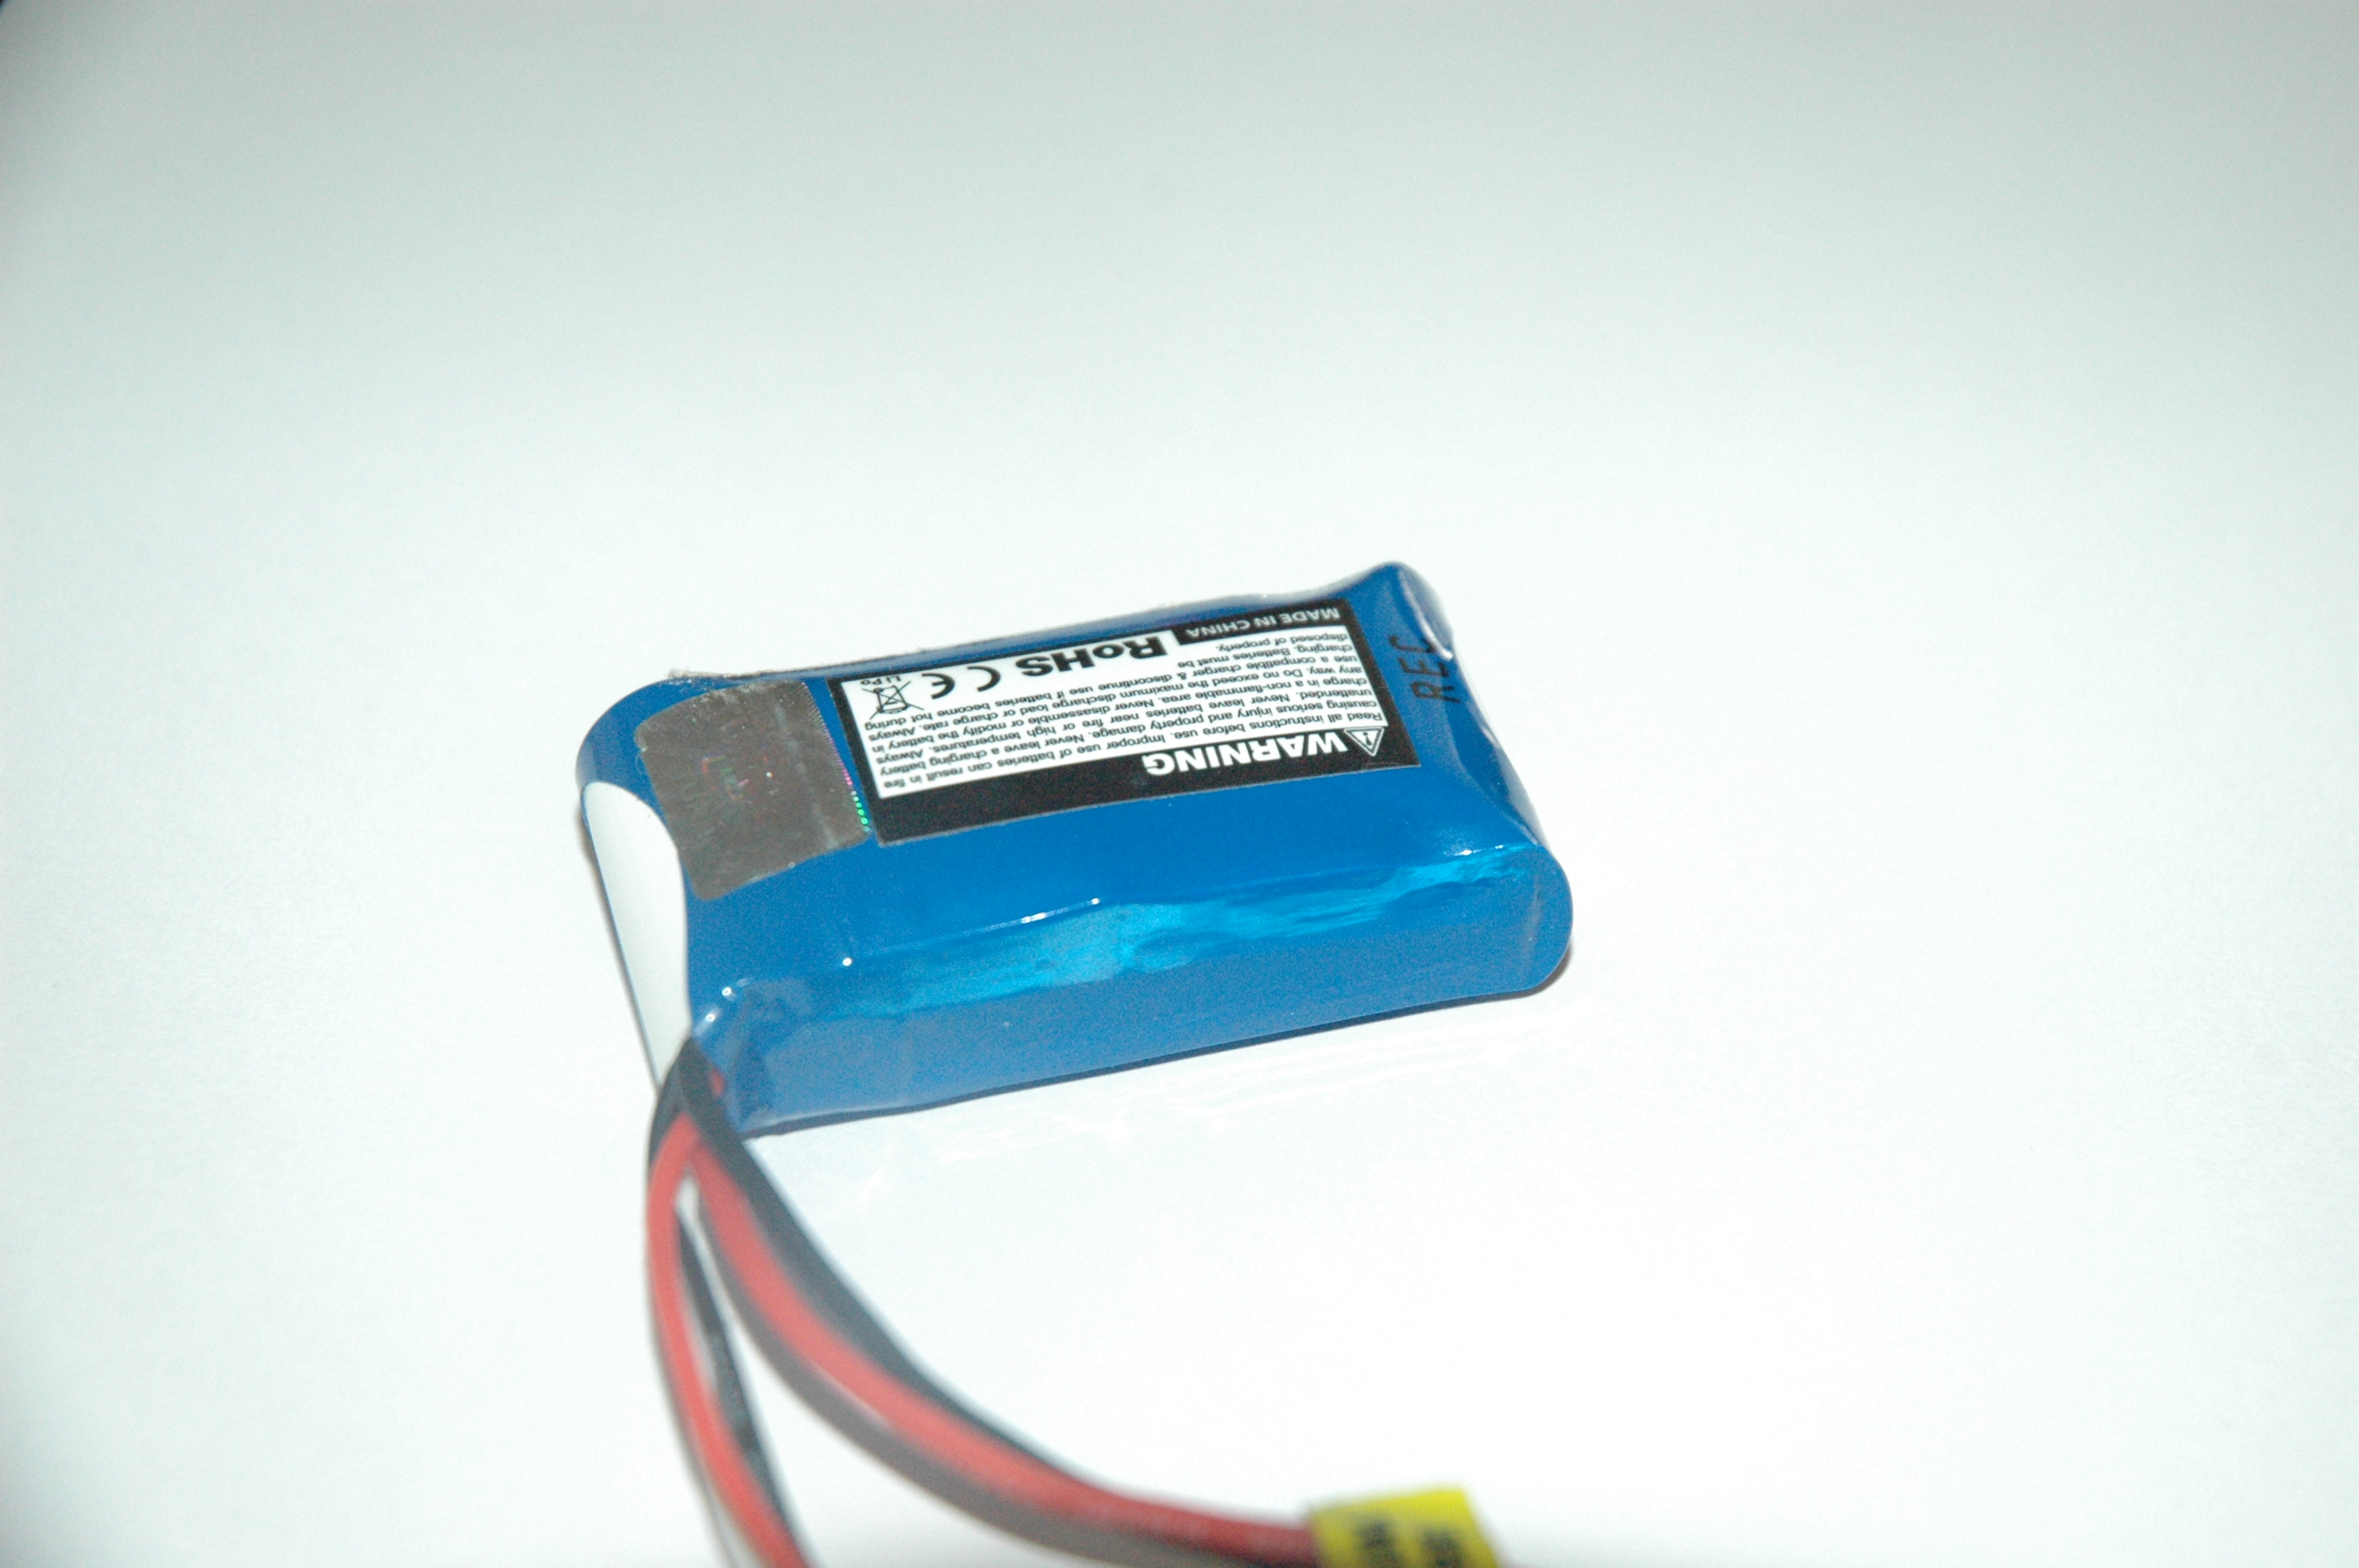
\includegraphics[width=0.75\linewidth]{danger_lipo}}
                    \vspace{10pt}
                    
                    To dispose of the LiPo, you soak it in a salty water solution for around 2 weeks.\\
                    
                    \centerline{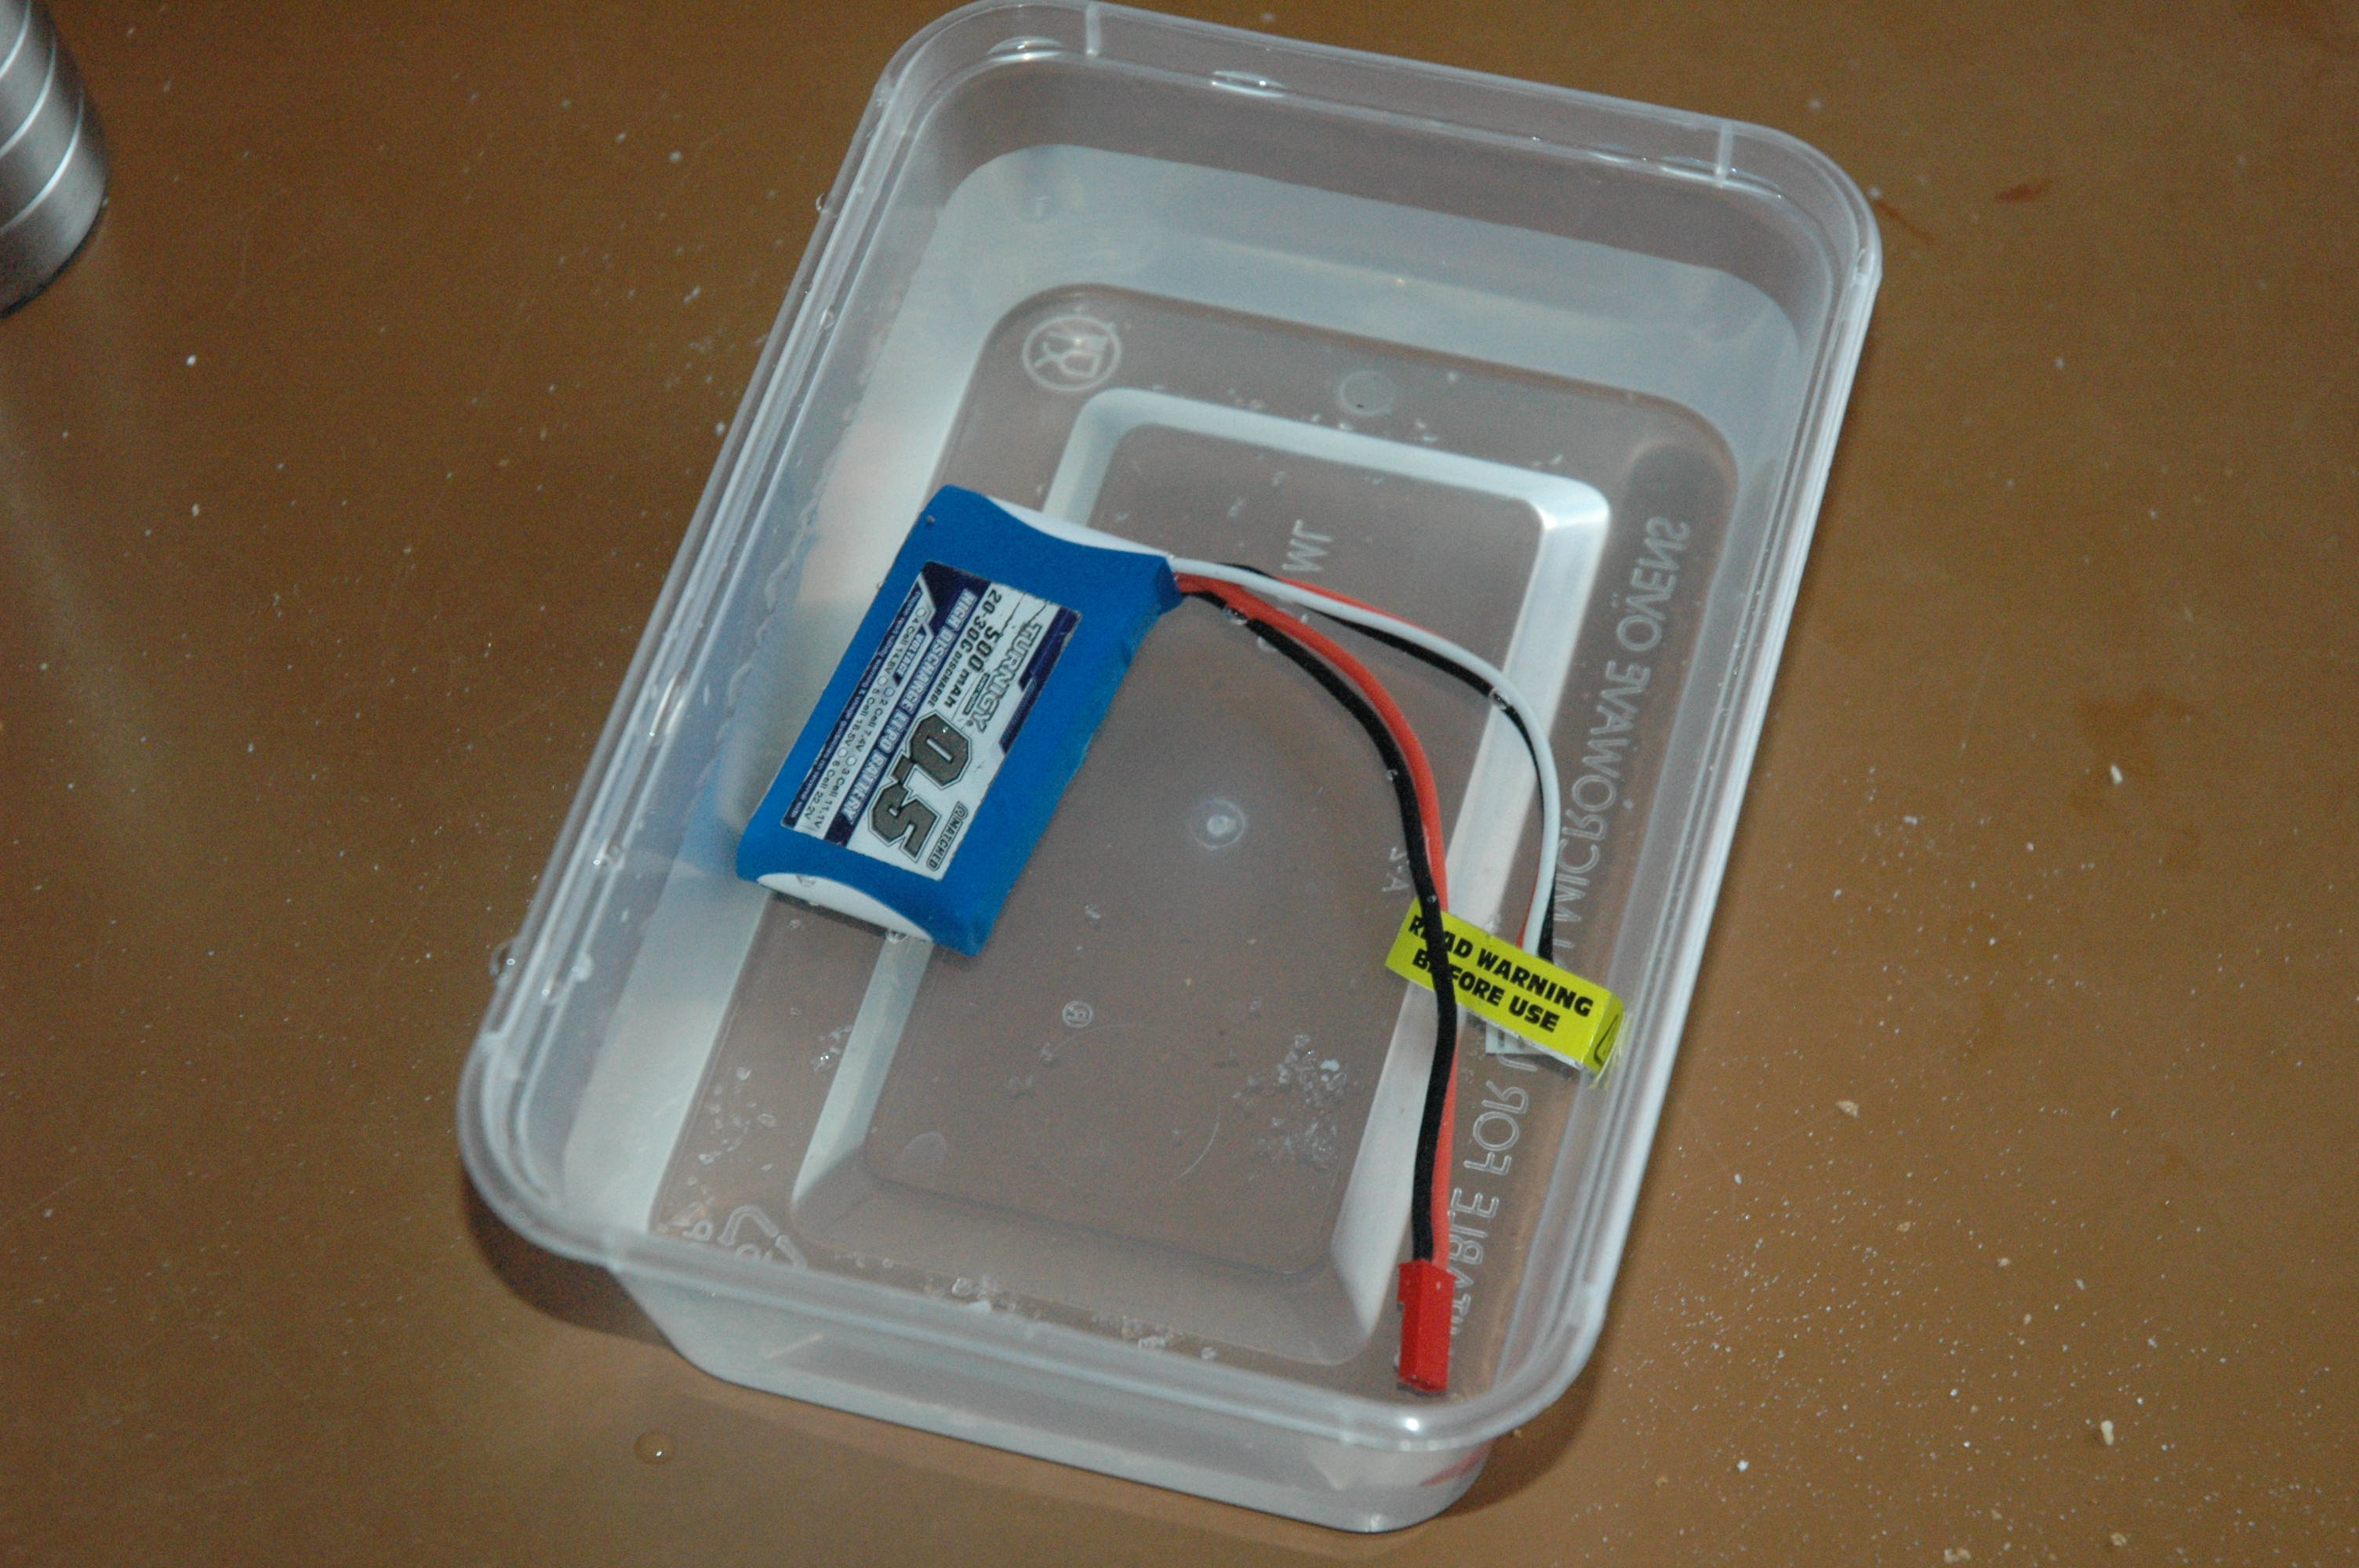
\includegraphics[width=0.75\linewidth]{lipo_dispose}}
                    \vspace{10pt}

